\documentclass[11pt]{article}

\pdfobjcompresslevel=3    % compress PDF objects
\pdfcompresslevel=9       % compress streams more (0..9)
\pdfminorversion=4


\usepackage[utf8]{inputenc} % remove if using XeLaTeX or LuaLaTeX
\usepackage[T1]{fontenc}

% Layout & graphics
\usepackage[a4paper, total={7.5in, 9in}]{geometry}
\usepackage{graphicx}              % images
\usepackage[dvipsnames,table]{xcolor} % single xcolor invocation (keeps table option)

% Math & symbols
\usepackage{amsmath}
\usepackage{amssymb}
\usepackage{gensymb}

% Typography & layout helpers

\usepackage{polski}[babel]

\usepackage{microtype}
\usepackage{float}                 %  placement
\usepackage{caption}
\usepackage{subcaption}            % modern subfigure support (do NOT load subfig)
\usepackage{multirow}
\usepackage{titlesec}

\usepackage{lmodern}
\usepackage{microtype}

\usepackage{pgfplots}
\usepackage{booktabs}
\usepackage{siunitx}
\pgfplotsset{compat=1.18}

\definecolor{xppblue}{RGB}{37, 150, 190}

\begin{document}

\begin{table}
    \centering
    \scalebox{1.5}{
        \begin{tabular}{|c|p{3cm}|l|l|cl|}
            \hline
            \multicolumn{4}{|c|}{SPRAWOZDANIE Z LABORATORIUM}                      & \multicolumn{2}{c|}{\multirow{2}{*}{\begin{tabular}[c]{@{}c@{}}rok akademicki:\\ 2025/26\end{tabular}}}                                                          \\ \cline{1-4}
            \multicolumn{4}{|c|}{\textbf{Układy elektroniki użytkowej}}            & \multicolumn{2}{c|}{}                                                                                                                                            \\ \hline
            \multicolumn{4}{|c|}{\multirow{2}{*}{\textit{Układy wejścia-wyjścia}}} & \multicolumn{2}{c|}{\multirow{2}{*}{czwartek 8:00}}                                                                                                              \\
            \multicolumn{4}{|c|}{}                                                 & \multicolumn{2}{c|}{}                                                                                                                                            \\ \hline
            \multicolumn{1}{|c|}{WARiE, AiR, sem 5}                                & \multicolumn{3}{p{5cm}|}{\begin{tabular}[c]{@{}l@{}}1. Piotr Cybal\\ \underline{2. Piotr Bednarek}\end{tabular}} & \multicolumn{2}{l|}{\multirow{2}{*}{Punkty:}} \\ \cline{1-1}
            \multicolumn{1}{|c|}{26.11.2025}                                       & \multicolumn{3}{c|}{}                                                                                            & \multicolumn{2}{l|}{}                         \\ \hline
        \end{tabular}
    }
\end{table}

\vspace{1\baselineskip}

\section*{Sprzęt}
\begin{itemize}
    \item Numer stanowiska: 8
    \item Numer Elvisa: E
    \item Numer skrzynki z elementami: 5
\end{itemize}

\section{Cel ćwiczenia}
Celem ćwiczenia było zapoznanie się z parametrami analogowych i cyfrowych linii
wejścia-wyjścia występujących w układach scalonych.

\section{Wejście cyfrowe}
W badaniu wykorzystano rezystor $10~\Omega$ o mocy $1~W$ oraz tolerancji 5\%.
Przy takich parametrach rezysotr może mieć rzeczywistą wartość od $9,5~\Omega$ do $10,5~\Omega$.
Ze względu na bardzo małe prądy, charakterystykę wyznaczono sumarycznie dla 4 wejść
połączonych równolegle.

\begin{figure}[H]
    \centering
    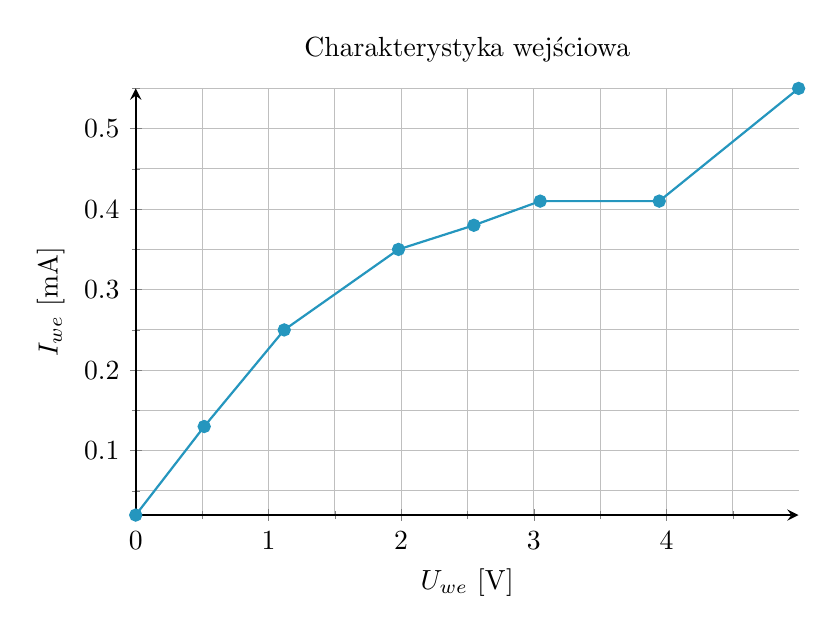
\begin{tikzpicture}
        \begin{axis}[
                width=10cm,
                height=7cm,
                xlabel={$U_{we}$ [\unit{\volt}]},
                ylabel={$I_{we}$ [\unit{\milli\ampere}]},
                grid=both,
                minor tick num=1,
                axis lines=left,
                thick,
                title={Charakterystyka wejściowa},
            ]
            \addplot[
                color=xppblue,
                mark=*,
                mark size=2pt
            ]
            coordinates {
                    (0,0.02)
                    (0.516,0.13)
                    (1.119,0.25)
                    (1.98,0.35)
                    (2.548,0.38)
                    (3.048,0.41)
                    (3.945,0.41)
                    (4.995,0.55)
                };
        \end{axis}
    \end{tikzpicture}
    \caption{Zależność prądu wejściowego od napięcia wejściowego}
    \label{fig:char_wej}
\end{figure}

Jak widać na charakterystyce wejściowej nie występuje histereza.

Parametry z noty katalogowej:
\begin{itemize}
    \item Próg narastający ($V_{T+}$): max $2,2~V$
    \item Próg opadający ($V_{T-}$): min $0,8~V$
    \item Histereza ($\Delta V_T$): min $0,2~V$
\end{itemize}

Zmierzone wartości:
\begin{itemize}
    \item Przełączenie $L \rightarrow H$: $1,635~V$
    \item Przełączenie $H \rightarrow L$: $1,446~V$
    \item Zmierzona histereza: $0,189~V$
\end{itemize}

\paragraph{Porównanie}

Zmierzona histereza jest mniejsza od minimalnej wartości z noty katalogowej, dzieje się
tak z powodu, połączenia równoległego 4 wejść. Wprowadzą to błędy pomiarowe, które
uszczuplają histerezę.

\paragraph{Czy występuje napięcie, przy którym wejścia DIOx, mimo równoległego połączenia, wskazują różne stany binarne?}

Tak, występuje, ponieważ rzeczywisty próg przełączania jest nieprecyzyjny i może się
różnić w zależności od wejścia.

\section{Wyjście analogowe}

Poniżej przedstawiono charakterystyki obciążenia wyjścia analogowego dla dwóch nastaw napięciowych: \SI{3}{\volt} oraz \SI{5}{\volt}.

\definecolor{xppred}{RGB}{190, 37, 37}


\begin{figure}[H]
    \centering
    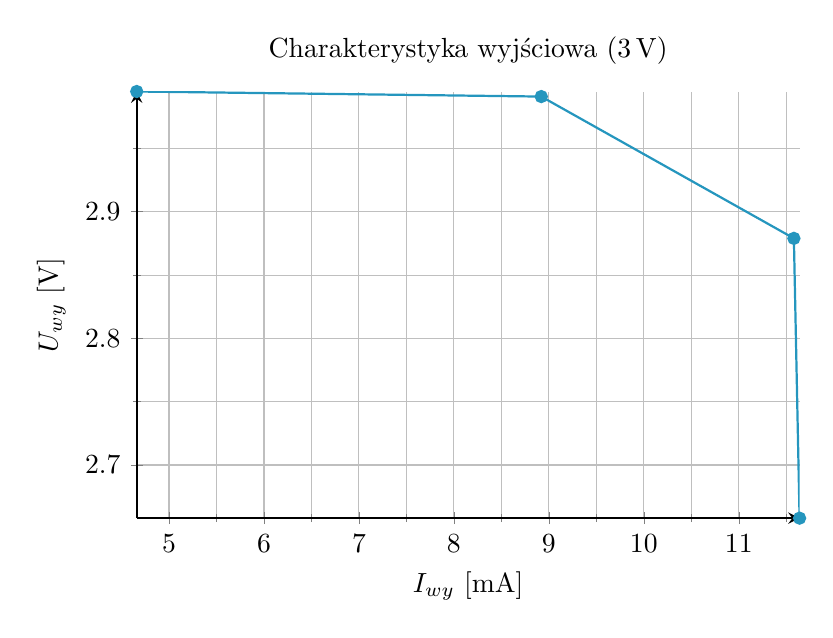
\begin{tikzpicture}
        \begin{axis}[
                width=10cm,
                height=7cm,
                xlabel={$I_{wy}$ [\unit{\milli\ampere}]},
                ylabel={$U_{wy}$ [\unit{\volt}]},
                grid=both,
                minor tick num=1,
                axis lines=left,
                thick,
                title={Charakterystyka wyjściowa (\SI{3}{\volt})},
            ]
            \addplot[
                color=xppblue,
                mark=*,
                mark size=2pt
            ]
            coordinates {
                    (4.66, 2.995)
                    (8.92, 2.991)
                    (11.58, 2.879)
                    (11.64, 2.658)
                };
        \end{axis}
    \end{tikzpicture}
    \caption{Zależność napięcia wyjściowego od prądu obciążenia dla \SI{3}{\volt}}
    \label{fig:char_wyj_analog_3v}
\end{figure}

\begin{figure}[H]
    \centering
    \begin{tikzpicture}
        \begin{axis}[
                width=10cm,
                height=7cm,
                xlabel={$I_{wy}$ [\unit{\milli\ampere}]},
                ylabel={$U_{wy}$ [\unit{\volt}]},
                grid=both,
                minor tick num=1,
                axis lines=left,
                thick,
                title={Charakterystyka obciążenia (\SI{5}{\volt})},
            ]
            \addplot[
                color=xppred,
                mark=square*,
                mark size=2pt
            ]
            coordinates {
                    (11.28, 4.567)
                    (11.66, 3.314)
                    (11.54, 2.875)
                    (11.60, 2.655)
                };
        \end{axis}
    \end{tikzpicture}
    \caption{Zależność napięcia wyjściowego od prądu obciążenia dla \SI{5}{\volt}}
    \label{fig:char_wyj_analog_5v}
\end{figure}

\begin{figure}[H]
    \centering
    \begin{tikzpicture}
        \begin{axis}[
                width=10cm,
                height=7cm,
                xlabel={$U_{nastawy}$ [\unit{\volt}]},
                ylabel={$U_{wy}$ [\unit{\volt}]},
                grid=both,
                minor tick num=1,
                axis lines=left,
                thick,
                legend pos=north west,
                title={Charakterystyka przejściowa wyjścia analogowego},
            ]

            % Wyjście nieobciążone (Idealne)
            \addplot[
                color=gray,
                dashed,
                domain=0:5,
                samples=2
            ]
            {x};
            \addlegendentry{Wyjście nieobciążone}

            % Wyjście obciążone (4 diody)
            \addplot[
                color=xppblue,
                mark=*,
                mark size=2pt
            ]
            coordinates {
                    (0.5, 0.5)
                    (1, 1)
                    (1.5, 1.5)
                    (2, 1.998)
                    (2.5, 2.491)
                    (3, 2.667)
                    (3.5, 2.657)
                    (4, 2.654)
                    (4.5, 2.654)
                    (5, 2.654)
                };
            \addlegendentry{Wyjście obciążone (4 diody)}

        \end{axis}
    \end{tikzpicture}
    \caption{Zależność napięcia wyjściowego od napięcia}
    \label{fig:char_przejsciowa_analog}
\end{figure}

\textbf{Parametry katalogowe:} Maksymalny prąd wyjściowy wynosi $\pm 5~mA$.

\textbf{Wyniki pomiarów:}
Zmierzone charakterystyki wykazują zadziałanie ogranicznika prądowego przy wartości ok.
$9~mA$. Jest to wartość wyższa od gwarantowanego maksimum przez producenta.
Widoczne jest
nasycenie napięcia wyjściowego na poziomie ok. $2,5~V$ przy większym obciążeniu, co wynika
z ograniczenia prądowego.

\section{Wyjście cyfrowe}

\begin{figure}[H]
    \centering
    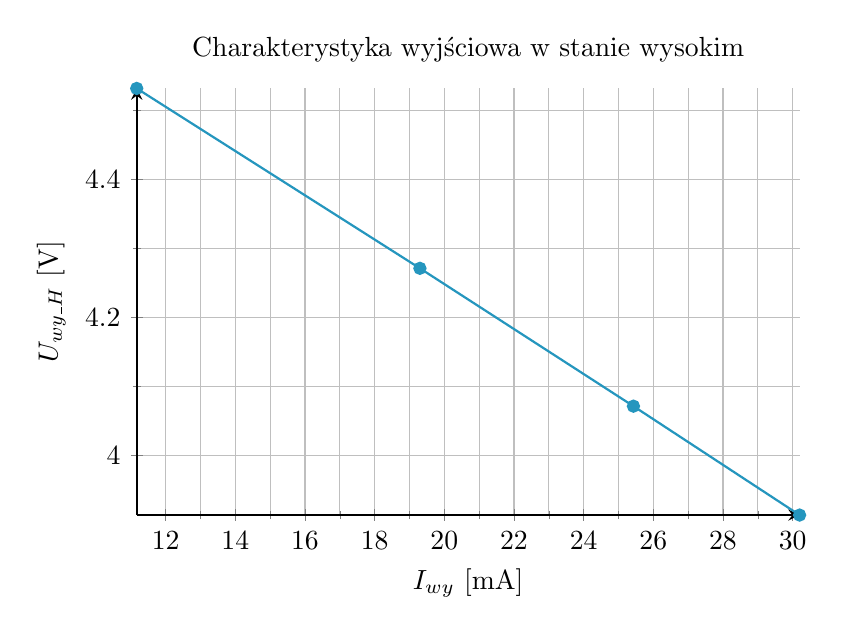
\begin{tikzpicture}
        \begin{axis}[
                width=10cm,
                height=7cm,
                xlabel={$I_{wy}$ [\unit{\milli\ampere}]},
                ylabel={$U_{wy\_H}$ [\unit{\volt}]},
                grid=both,
                minor tick num=1,
                axis lines=left,
                thick,
                title={Charakterystyka wyjściowa w stanie wysokim},
            ]
            \addplot[
                color=xppblue,
                mark=*,
                mark size=2pt
            ]
            coordinates {
                    (11.17, 4.532)
                    (19.3, 4.271)
                    (25.43, 4.071)
                    (30.2, 3.913)
                };
        \end{axis}
    \end{tikzpicture}
    \caption{Zależność napięcia wyjściowego w stanie wysokim od prądu obciążenia}
    \label{fig:char_wyj_cyf_H}
\end{figure}

\begin{figure}[H]
    \centering
    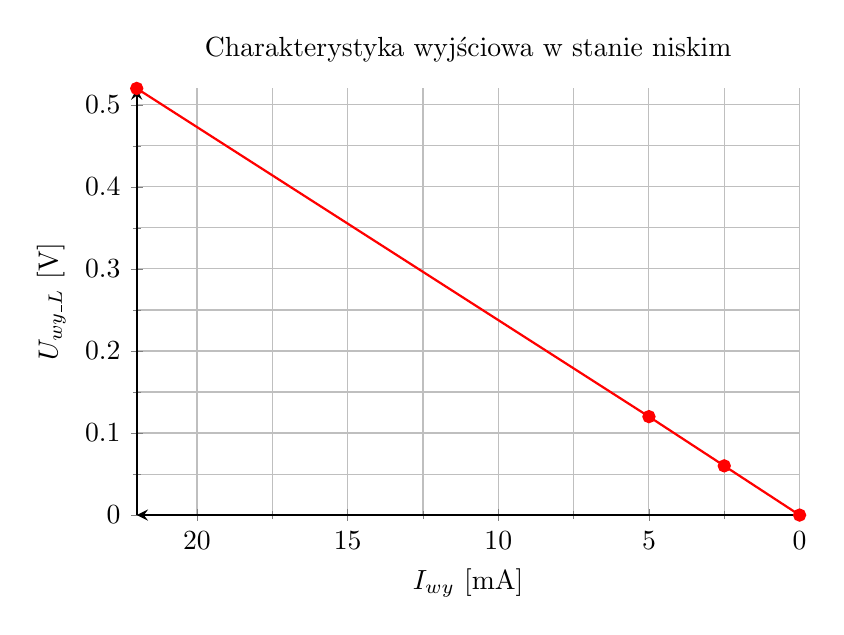
\begin{tikzpicture}
        \begin{axis}[
                width=10cm,
                height=7cm,
                xlabel={$I_{wy}$ [\unit{\milli\ampere}]},
                ylabel={$U_{wy\_L}$ [\unit{\volt}]},
                grid=both,
                minor tick num=1,
                axis lines=left,
                thick,
                title={Charakterystyka wyjściowa w stanie niskim},
                x dir=reverse,
            ]
            \addplot[
                color=red,
                mark=*,
                mark size=2pt
            ]
            coordinates {
                    (0, 0.0)
                    (2.5, 0.06)
                    (5.0, 0.12)
                    (22.0, 0.52)
                };
        \end{axis}
    \end{tikzpicture}
    \caption{Zależność napięcia wyjściowego w stanie niskim od prądu wpływającego}
    \label{fig:char_wyj_cyf_L}
\end{figure}

\paragraph{Parametry z noty katalogowej (NI ELVIS II):}
\begin{itemize}
    \item Maksymalny prąd wyjściowy ($I_{OH}/I_{OL}$): \SI{24}{\milli\ampere}
\end{itemize}

\paragraph{Porównanie i wnioski}
Liniowy kształt wyznaczonych charakterystyk potwierdza rezystancyjny charakter wyjść
cyfrowych.


\textbf{W stanie wysokim:} Zmierzone napięcia mieszczą się w specyfikacji. Nawet przy
prądzie rzędu \SI{30}{\milli\ampere}, co przekracza nominalny prąd
(\SI{24}{\milli\ampere}), napięcie utrzymywało się na wysokim poziomie ok. \SI{3.9}{\volt}.

\textbf{W stanie niskim:} Przy obciążeniu prądem ok. \SI{22}{\milli\ampere} (blisko
granicy katalogowej), napięcie na wyjściu wzrosło do \SI{0.52}{\volt}. Jest to wartość
bezpieczna, mieszcząca się w standardowym zakresie logicznego "zera".

\section{Wejście liczników cyfrowych}

\paragraph{W jakim stanie ustalają się niepodłączone wejścia cyfrowe liczników?}
Niepodłączone wejścia w standardzie TTL ustalają się w stanie logicznym niskim (Low).
W technologii CMOS stan jest teoretycznie nieokreślony, lecz
w układzie ELVIS często wymuszany jest stan wysoki przez rezystory ściągające.

\paragraph{Czy ta zasada jest wspólna dla różnych rodzin układów (TTL/CMOS)?}
Nie, wejścia TTL samoczynnie przyjmują stan wysoki, natomiast wejścia CMOS charakteryzują
się wysoką impedancją. Pozostawienie wejścia CMOS bez potencjału jest błędem projektowym,
który może prowadzić do oscylacji lub uszkodzenia układu.

\paragraph{Przetestować włączanie powolne i szybkie. Czy (i jakie) występują różnice?}
Tak, przy powolnym przełączaniu drgania styków trwają dłużej, co powoduje zliczenie
większej liczby fałszywych impulsów przez szybki licznik sprzętowy. Szybki
ruch włącznikiem skraca czas drgań, redukując liczbę błędnych zliczeń.

\paragraph{Czy liczniki równo zliczają impulsy?}
Nie, liczniki nie zliczają równo. Licznik sprzętowy (PFI) rejestruje znacznie więcej
impulsów niż wolniejszy licznik programowy (DIO), który pomija większość drgań.

\paragraph{Jeżeli nie, to co jest tego przyczyną?}
Przyczyną jest zjawisko drgania styków (bouncing), które generuje serię krótkich impulsów
napięciowych podczas jednego przełączenia. Licznik sprzętowy o wysokiej częstotliwości
próbkowania (80 MHz) interpretuje każde drganie jako osobny impuls.

\paragraph{Jakie zdarzenie zliczają liczniki: stan niski, stan wysoki, zmianę stanu z
    niskiego na wysoki ($L\uparrow H$), czy wysokiego na niski ($H\downarrow L$)?}
Liczniki są skonfigurowane na zliczanie zbocza narastającego ($L\uparrow H$).
Obserwowane wielokrotne zliczenia przy zmianie $H\downarrow L$ wynikają z
faktu, że drgania styków powodują wielokrotne powroty sygnału powyżej i poniżej progu
przełączania.

\paragraph{(Po modyfikacji układu) Czy liczniki równo zliczają impulsy?}
Tak, przy szybkim przełączaniu liczniki zliczają równo, ponieważ kondensator eliminuje
drgania napięcia. Przy bardzo wolnym przełączaniu mogą nadal wystąpić drobne
różnice, jeśli czas narastania zbocza jest zbyt wolny dla układu wejściowego.
\paragraph{Stała RC układu dla $L\uparrow H$:}
Podczas ładowania rezystancja zastępcza to $R_1 || R_2$, co daje: $\tau = \frac{R_1
        R_2}{R_1+R_2} \cdot C \approx 1,67 k\Omega \cdot 100 nF = 167 \mu s$.

\paragraph{Stała RC układu dla $H\downarrow L$:}
Podczas rozładowania prąd płynie tylko przez $R_2$, więc: $\tau = R_2 \cdot C = 10 k\Omega
    \cdot 100 nF = 1000 \mu s = 1 ms$.

\paragraph{Minimalny czas impulsu dla licznika sprzętowego:}
Dla licznika w układzie NI ELVIS II (bazującego na zegarze 80 MHz) minimalny czas trwania
impulsu wynosi $12,5 ns$.

\paragraph{Dlaczego zachowanie liczników jest inne niż w p. 5?}
Dodanie kondensatora tworzy filtr dolnoprzepustowy, który wygładza gwałtowne skoki
napięcia spowodowane drganiami styków. Sygnał narasta wykładniczo,
przekraczając próg logiczny tylko raz, co eliminuje fałszywe zliczenia.

\paragraph{Czy do tłumienia drgań styków można użyć innego rozwiązania niż na rys. 7?}
Tak, powszechnie stosuje się rowiązania sprzętowe jak i programowe metody debouncingu
(opóźnienie czasowe po wykryciu pierwszego zbocza).

\section{Wnioski końcowe}

Na podstawie przeprowadzonych eksperymentów sformułowano dwa kluczowe wnioski:

\begin{enumerate}
    \item \textbf{Konieczność eliminacji drgań styków w układach cyfrowych:}
          Bezpośrednie podłączenie styków mechanicznych do szybkich liczników cyfrowych
          prowadzi do błędów w działaniu systemu, ponieważ każdy ruch styku generuje serię
          niepożądanych impulsów (zjawisko \textit{bouncingu}). Aby zapewnić poprawne
          zliczanie, niezbędne jest zastosowanie układów kondycjonujących sygnał –
          najprostszym i skutecznym rozwiązaniem sprzętowym jest filtr dolnoprzepustowy RC
          (układ całkujący), który spowalnia narastanie zbocza i eliminuje stany
          nieustalone, zapewniając pojedyncze, czyste przełączenie logiczne.

    \item \textbf{Fundamentalna różnica charakterystyk wyjść analogowych i cyfrowych:}
          Wyjścia cyfrowe zachowują się jak źródła napięciowe z szeregową rezystancją
          (liniowy spadek napięcia pod obciążeniem), pozwalając na pobór prądu rzędu 24-30
          mA przy jedynie pogorszeniu poziomów napięć. Natomiast wyjścia analogowe
          posiadają sztywne, aktywne ograniczenie prądowe (w badanym układzie ok. 9 mA).
          Przekroczenie tej wartości powoduje gwałtowne „obcięcie” napięcia wyjściowego,
          co sprawia, że wyjście analogowe nie nadaje się do bezpośredniego sterowania
          elementami wykonawczymi o niskiej rezystancji, w przeciwieństwie do wyjść
          cyfrowych.
\end{enumerate}

\end{document}
